\chapter{I filtri di Bloom}

\section{Strutture dati e algoritmi probabilistici}

Le strutture dati e gli algoritmi che basano il proprio funzionamento sull'utilizzo di una componente
di casualità vengono detti ``probabilistici''. 

Ci sono due principali famiglie di algoritmi probabilistici:

\begin{itemize}
	\medskip

	\item Gli algoritmi detti ``Monte Carlo'', nei quali si effettua un campionamento casuale di
	valori in uno spazio di ricerca, consentendo il calcolo approssimato entro una certa
	probabilità. Il nome deriva dal Principato di Monte Carlo, conosciuto a livello mondiale come
	meta per il gioco d'azzardo. Gli algoritmi di questo tipo permettono solitamente di bilanciare
	il tempo di esecuzione con l'errore richiesto, poiché aumentando il numero di tentativi l'errore
	scende. Un esempio di questi algoritmi sono i test di primalità (cioè i test per verificare se
	un numero è primo) come il test di Fermat, nei quali si effettua controlli di una condizione
	necessaria ma non sufficiente e ci si convince che il numero è il primo quando con un
	determinato numero di tentativi.

	\item Gli algoritmi detti ``Las Vegas'', nei quali si utilizza la casualità durante l'algoritmo,
	ma viene prodotto sempre un risultato esatto, oppure l'algoritmo fallisce esplicitamente
	l'esecuzione. In questo caso dunque la componente casuale non è parte integrante della qualità
	risultato ottenuto, ma può influenzare il tempo d'esecuzione. Un esempio classico è l'algoritmo
	di ordinamento ``Quicksort'' in cui la scelta del pivot da utilizzare ad ogni passaggio è
	casuale, ma il risultato è sempre corretto. Il nome è stato proposto in \cite{lasvegas} per
	contrasto con Monte Carlo, dato che Las Vegas è un'altra meta conosciuta per il gioco d'azzardo.
\end{itemize}

Nelle strutture dati, invece, l'utilizzo del caso permette la memorizzazione di un'informazione
parziale, consentendo comunque di elaborarla almeno parzialmente ma con margini di errori
accettabili. Si tratta tipicamente di strutture dati molto specialistiche, utili ad implementare un
solo specifico algoritmo, poiché la perdita di informazione controllata è orientata a memorizzare il
minimo indispensabile per lo specifico scenario d'uso, ma impedendo ovviamente delle operazioni che
richiedono l'informazione completa, come anche la semplice enumerazione.

\section{Gli insiemi}

Un insieme è una struttura dati che memorizza un gruppo di elementi distinti, senza alcun ordine tra
essi (quindi né ordinamento intrinseco dei dati, né ordinamento esterno quale per esempio l'ordine
di inserimento).

Le operazioni principali che si possono effettuare sulla struttura dati sono le seguenti:

\begin{itemize}
	\medskip

	\item
	\textbf{Inserimento}: aggiunge un elemento all'insieme. Se l'elemento è già presente,
	l'operazione non modifica la struttura dati. In alcune implementazioni, l'operazione può 
	restituire un codice di errore per indicare che l'inserimento non è stato effettuato
	perché l'elemento era già presente.

	\item
	\textbf{Test di appartenenza}: controlla se un elemento è presente nell'insieme.

	\item
	\textbf{Cardinalità}: restituisce il numero di elementi presenti nell'insieme.

	\item
	\textbf{Unione}: restituisce un insieme che contiene tutti gli elementi presenti in almeno uno
	degli insiemi forniti in ingresso.

	\item
	\textbf{Intersezione}: restituisce un insieme che contiene tutti gli elementi presenti in tutti
	gli insiemi forniti in ingresso.
\end{itemize}

Alcune implementazioni offrono anche operazioni più avanzate legate alla teoria degli insiemi,
come per esempio la differenza o la differenza simmetrica. 

Un'implementazione classica di un'insieme prevede l'utilizzo di una tabella hash: l'inserimento
di un elemento avviene codificandolo con una funzione hash, memorizzandolo all'interno della
tabella, gestendo in modo opportuno le collisioni; il test di appartenenza può essere fatto così in
modo efficiente effettuando una ricerca nella tabella hash. Entrambe queste operazioni così 
implementate richiedono quindi un tempo d'esecuzione ammortizzato costante ($\mathcal{O}(k)$).

Al contrario di un array associativo, un insieme non ha dati associati all'elemento stesso, ma
nonostante questo è spesso possibile riutilizzare la stessa implementazione di tabella hash,
associando un dato nullo (non significativo) all'elemento. Questo accade comunemente nei linguaggi e
nelle librerie che mettono a disposizione una struttura dati di tipo array associativo (poiché più
completa); per esempio, il linguaggio Python fin dalla versione 1.0 prevedeva il ``dizionario'' come
struttura dati (un array associativo implementato con tabella hash), mentre l'``insieme'' è stato
aggiunto nella versione 2.3; prima di allora, era comune implementare l'insieme con un dizionario i
cui valori erano semplicemente valori booleani (di solito \verb|True|).

\section{Proprietà dei filtri di Bloom}

Un filtro di Bloom \cite{bloomfilters} è una rappresentazione probabilistica di un insieme. Nel
filtro infatti non vengono memorizzati per intero tutti gli elementi, ma ne viene memorizzata solo
una rappresentazione parziale, che consente di effettuare comunque alcune operazioni, mantenendo
però dei margini di errore controllati.

In particolare, il test di appartenenza restituisce un valore probabilistico, con la presenza di
falsi valori positivi (cioè il test restituisce un valore di successo anche per elementi non
effettivamente presenti). Il margine di errore può essere controllato tramite alcuni parametri, che
vengono stabiliti al momento della creazione del filtro stesso.

Vediamo nel dettaglio come i filtri si comportano relativamente alle operazioni principali sugli
insiemi elencate precedentemente:

\begin{itemize}
	\medskip

	\item
	\textbf{Inserimento}: è possibile inserire un elemento in un filtro, fino ad un numero massimo
	di elementi calcolabile in base ai parametri del filtro stesso. I filtri non possono essere
	infatti ridimensionati dopo la creazione e quando raggiungono il numero massimo di elementi,
	l'aggiunta di ulteriori elementi, seppure tecnicamente possibile, aumenta esponenzialmente 
	il margine di errore, rendendo di fatto il filtro inutilizzabile.

	Durante l'inserimento, è possibile effettuare contemporaneamente un test di appartenenza,
	restituendo una informazione probabilistica se l'elemento inserito era già presente o meno.

	\item
	\textbf{Test di appartenenza}: il filtro è in grado di verificare se un elemento è stato
	inserito con un certo margine di errore. In particolare, se il test restituisce un valore
	positivo, l'elemento è \emph{probabilmente presente}, con una soglia di errore controllato;
	ciò vuol dire che non si può avere la certezza che l'elemento sia effettivamente presente
	nell'insieme. Viceversa, se il test restituisce un valore negativo, si ha la certezza che il
	valore non è presente nell'insieme.

	\item
	\textbf{Cardinalità}: il filtro è in grado di effettuare una stima della cardinalità, compiendo
	un errore controllato sul valore restituito. I risultati rimangono consistenti anche al crescere
	della densità.

	\item
	\textbf{Unione}: è possibile calcolare con precisione l'unione di due filtri, purché siano
	creati con gli stessi parametri. Si noti che l'unione risultante dovrà rispettare il limite
	massimo di elementi previsto dai parametri di creazione, altrimenti non sarà utilizzabile.

	\item
	\textbf{Intersezione}: è possibile calcolare con precisione l'intersezione di due filtri,
	purché siano creati con gli stessi parametri.

\end{itemize}

\section{Scenari applicativi}

I filtri di Bloom hanno conosciuto negli anni una ampia adozione, in diversi scenari applicativi. 
In linea generale, consentono di ottenere una rappresentazione compatta di un insieme di dati,
che può essere usata sia come cache ad accesso veloce (in RAM) per un controllo preliminare
di esistenza di un elemento, sia trasferita in modo efficiente via rete ad un altro nodo per
fornire una vista parziale di un set di dati.

Un approfondimento degli scenari applicativi presentati qui può essere trovata in
\cite{bloom-network}.

\subsection{Controllo ortografico e sillabazione}

Quando furono introdotti nel 1970, Bloom stava lavorando ad un programma per la sillabazione del
testo inglese. Al contrario delle lingue latine, la sillabazione delle parole nella lingua inglese 
non è basata sui fonemi, ma sull'etimologia o la morfologia delle parole. Questo rende le regole
di sillabazione molto complesse, con numerose eccezioni. Bloom pensò di ottimizzare il programma
utilizzando un filtro per memorizzare tutte le parole che richiedevano un'eccezione; il programma
poteva così verificare velocemente se una parola era soggetta ad eccezione o meno con un test
di appartenenza nel filtro; nel caso il test restituisse un valore positivo, il programma poteva
effettuare un controllo più lento nel dizionario completo delle eccezione. Le parole soggette
a falso positivo venivano riportate al caso standard al termine del controllo nel dizionario.

Allo stesso modo, i filtri di Bloom vennero usati per i primi programmi di controllo ortografico
negli anni 80. Era possibile infatti memorizzare una versione compatta di un dizionario di tutte le
parole conosciute (complete anche tutte le forme verbali che possono essere costruite tramite
algoritmo), ed utilizzarlo per effettuare il controllo; in questo caso, i falsi positivi
corrispondevano a parole non esistenti che veniva erroneamente ignorate durante il controllo. Visto
che all'epoca non era possibile distribuire l'intero dizionario, questa soluzione era un compromesso
accettabile.

\subsection{Proxy Cache distribuita}

In \cite{bloom-proxy}, viene introdotto uno dei primi casi di utilizzo dei filtri di Bloom per
ottimizzare i trasferimenti di rete. Lo scenario prevedeva una rete di proxy web, che comunicavano
tra loro. Nel momento in cui veniva effettuata una richiesta ad un proxy per una pagina web non
presente nella cache, il proxy poteva comunicare con gli altri proxy della rete, chiedendo loro
se qualcuno aveva nella propria cache la pagina richiesta, in modo da accedervi senza contattare
il server d'origine.

Per diminuire il traffico generato per la comunicazione tra proxy, fu introdotto un meccanismo
tramite il quale ciascun proxy periodicamente pubblicava in broadcast un filtro di Bloom contenente
l'elenco dei siti memorizzati nella propria cache. Gli altri proxy memorizzavano il filtro e
potevano usarlo per verificare se un sito era presente in cache senza causare traffico di rete. I
falsi positivi corrispondevano dunque a richieste di rete potenzialmente inutili, ma in ogni caso
una piccola frazione rispetto alla quantità di traffico generato in precedenza per ogni richiesta.


\subsection{Google SafeBrowsing}

Il browser Chrome di Google utilizzava (fino al 2012) i filtri di Bloom per implementare
efficientemente la funzionalità \fnhref{https://safebrowsing.google.com}{``SafeBrowsing''}, che
protegge gli utenti bloccando automaticamente l'accesso ai siti contenenti \emph{malware} o
\emph{phishing}.

Google, infatti, mantiene sui propri server un enorme elenco di tipo \emph{blacklist} di indirizzi
web (URL) considerate pericolose per gli utenti. L'elenco è in continua evoluzione: nuovi indirizzi
vengono infatti aggiunti e rimossi con alta frequenza ogni ora.

Un applicativo che volesse verificare la presenza di un sito all'interno dell'elenco potrebbe
effettuare una interrogazione via API ai server di Google; il tempo di esecuzione di questo
controllo comprende però almeno 1 \emph{roundtrip} di rete tra il client e il server, che può
richiedere tempi variabile a seconda della qualità della connessione Internet, ma può salire fino a
centinaia di millisecondi per una connessione mobile (anche in presenza di segnale ottimale). Questo
genere di attesa prima della visualizzazione di una pagina è considerato non accettabile per un
browser come Google Chrome, il quale cerca di minimizzare il tempo di apertura dei siti.

Scaricare l'intera lista di siti richiederebbe probabilmente molta banda, soprattutto per le
numerose sincronizzazione che sarebbero necessarie periodicamente. Vista l'alta volatilità della
lista, infatti, sarebbe necessario effettuare sincronizzazioni con alta frequenza, per evitare di
consultare una lista troppo vecchia, e questi aggiornamenti avrebbero impatti importanti
sull'utilizzo di banda Internet da parte del client.

La soluzione che fu scelta inizialmente fu quella di affidarsi ad un filtro di Bloom: i server
di Google infatti costruivano un filtro contenente tutte le URL presenti nella blacklist, e
trasferivano il filtro al client. Grazie alle proprietà dei filtri di Bloom, i dati da trasferire
erano molto compatti, e potevano essere conservati in RAM anche sui dispositivi mobili.

Ogni volta che l'utente navigava su un nuovo sito, il client verificava prima se l'indirizzo era
presente nel filtro: nel caso più comune (sito non malevole), il filtro restituiva correttamente
esito negativo, e il browser consentiva l'accesso all'utente senza nessun rallentamento. Solo nei
casi in cui il filtro restituiva esito positivo, il client effettuava una chiamata alle API di
Google per verificare se l'indirizzo era veramente malevolo o se si trattasse di un falso positivo;
con parametri di creazione adeguati, era possibile fare in modo che questa chiamata avvenisse
pochissime volte nel corso di una navigazione normale, impattando così il meno possibile i tempi
di apertura dei siti.

Con il passare del tempo, la lista è cresciuta troppo, e di conseguenza il filtro ha iniziato
ad avere dimensioni importanti; di conseguenza, è stato scelto di usare un'altra struttura dati
probabilistica (gli insiemi di Golomb-Rice \cite{golomb,rice,golomb-rice}), che ha una rappresentazione in memoria
compressa, dunque più compatta, sebbene più lenta da utilizzare \cite{golomb-safebrowsing}. 

\subsection{Riconciliazione di una rete di distribuzione contenuti}
\label{sec:bloomcdn}

Le reti di distribuzione contenuti (\emph{Content Delivery Network} o \emph{CDN}) sono delle reti
di server distribuiti geograficamente che memorizzano copie di dati statici (immagini, font, 
fogli di stile, sorgenti javascript) richiesti durante la navigazione di siti ad alto traffico. 
Memorizzando una copia di questi contenuti sui nodi della CDN, il contenuto può essere offerto
al visitatore da un server geograficamente più vicino a lui e quindi con una latenza di rete
inferiore, migliorando la velocità di accesso al sito; inoltre, il traffico si distribuisce
così su tanti nodi, diminuendo l'impatto del traffico sul server principale.

In alcuni casi, può essere richiesto che i nodi della CDN si \emph{riscaldino}, popolando le
proprie cache di contenuti che si ritiene verranno richiesti a breve dagli utenti. In questo caso,
le CDN lavorano con una logica di rete P2P, trasferendo i dati da nodo a nodo. Per sincronizzare
il contenuto del nodo $N1$ con il nodo $N2$, $N1$ invia a $N2$ un filtro di Bloom contentente
l'elenco dei contenuti presenti nella propria cache. $N2$ può quindi utilizzare il filtro
per individuare i contenuti che $N1$ non possiede, ed inviargieli. In caso di falso positivo,
un dato risulterà erroneamente posseduto da $N1$ e non verrà quindi inviato; trattandosi di una
operazione di ottimizzazione del traffico, è sufficiente che non avvenga con frequenza troppo 
elevata per non impattare sulle prestazioni: infatti $N1$ non avrà il dato disponibile all'arrivo
della prima richiesta, e si occuperà di scaricarlo in quel momento. 

L'azienda Akamai (leader di mercato nel settore delle CDN) utilizza i filtri di Bloom anche per
evitare di memorizzare contenuti richiesti una sola volta (come descritto in \cite{bloom-akamai}).
Infatti ogni nodo conserva un filtro di Bloom dei contenuti richiesti almeno una volta. Alla prima
richiesta, il contenuto non è ancora presente nel filtro e viene aggiunto ma non viene cachato
dal nodo. In questo modo, si evita di inserire in cache contenuti non popolari che possono 
utilizzare spazio meglio utilizzato da contenuti più richiesti. I falsi positivi corrispondono
a contenuti richiesti la prima volta che risultano però già richiesti; in questo caso, poiché
la probabilità è bassa, l'ottimizzazione ha comunque successo nel non appesantire troppo la cache.

\subsection{Routing ottimale in reti P2P}

All'interno delle reti puramente P2P, il routing è l'algoritmo che consente ad ogni nodo di
decidere verso quale altro nodo inviare un pacchetto. È possibile pensare alla rete P2P come
ad un grafo, e al problema del routing come alla ricerca di un percorso tra nodi all'interno
del grafo. La ricerca del percorso ottimale è di solito possibile tramite dei protocolli di 
\emph{path discovery}, che sono però abbastanza onerosi. Di conseguenza, è possibile memorizzare
l'esito della ricerca del percorso all'interno di un bloom filter associato ad ogni arco uscente.
Se viene richiesto di effettuare lo stesso routing, il bloom filter consente di individuare
rapidamente l'arco da utilizzare per inviare il pacchetto. I falsi positivi in questo caso
corrispondono a routing non ottimali: il pacchetto viene inviato erroneamente al nodo sbagliato,
ma probabilmente raggiungerà comunque poi la destinazione, sebbene non nel modo più efficiente. 

Le reti P2P sono per loro stessa natura dinamiche: i nodi si connettono e sconnettono con una certa
frequenza. Quando un nodo si disconnette, i nodi collegati possono decidere di buttare via il
filtro associato all'arco che scompare, o in alternativo unirlo ad un altro filtro di un nodo
magari ad alto traffico con molta banda a disposizione (utilizzando l'operazione di unione
dei filtri).

\section{Funzionamento dei filtri}

Un filtro di Bloom è un array di bit, utilizzato come tabella hash, di dimensione arbitraria
\verb|M| fissata al momento della creazione in base ai parametri (vedi la \autoref{sec:bloomparms}).
Quando il filtro è vuoto, tutti i bit sono impostati a 0. La seguente tabella mostra un filtro
vuoto composto di 11 bit:

\begin{center}
  \begin{tabular}{*{11}{|c}|}
  	\multicolumn{1}{c}{0} & \multicolumn{1}{c}{1} & \multicolumn{1}{c}{2} &
  	\multicolumn{1}{c}{3} & \multicolumn{1}{c}{4} & \multicolumn{1}{c}{5} &
  	\multicolumn{1}{c}{6} & \multicolumn{1}{c}{7} & \multicolumn{1}{c}{8} &
  	\multicolumn{1}{c}{9} & \multicolumn{1}{c}{10} \\
    \hline
    0 & 0 & 0 & 0 & 0 & 0 & 0 & 0 & 0 & 0 & 0 \\
    \hline
  \end{tabular}
\end{center}

\subsection{Inserimento di un elemento}
\label{sec:bloom:add}

L'inserimento di un elemento $X$ (\autoref{alg:bloominsert}) avviene calcolando alcune
funzioni di hash $h_i(X)$ prestabilite sull'elemento (il numero delle funzioni, chiamato $K$, è
anch'esso un parametro del filtro). I $K$ valori risultanti $h_0(X), h_1(X), ... , h_{K-1}(X)$ sono
utilizzati per identificare singoli bit all'interno dell'array (per esempio, scegliendo il bit con
indice $h_i(X) \bmod M$), e i bit così identificati vengono impostati a 1. Si noti che nessuna altra
informazione sull'elemento viene memorizzata dentro il filtro.

\begin{algorithm}
\caption{Inserimento elemento in filtro}
\label{alg:bloominsert}
\begin{algorithmic}[1]
\Procedure{BloomInsert}{$bf$, $x$}
	\For {$i=0$ \textbf{to} $K-1$}
		\State $j \gets h_i(x) \bmod M$
		\State $bf(j) \gets 1$
	\EndFor
\EndProcedure
\end{algorithmic}
\end{algorithm}

Continuando l'esempio seguente, supponiamo di utilizzare $K=2$ funzioni di hash $h_1(x)$ e $h_2(x)$
e di voler inserire 3 elementi $\{ A, B, C \}$ nel filtro. La seguente tabella mostra i valori
delle funzioni di hash per ciascun elemento:

\begin{center}
	\begin{tabular}{ l c c c }
		 & A & B & C \\
		\hline
		$h_1(x)$ & 1 & 10 & 7 \\
		$h_2(x)$ & 8 & 4 & 1 \\	
		\hline
	\end{tabular}
\end{center}

Per inserire l'elemento $A$, è dunque sufficiente impostare ad 1 i bit $h_1(A) = 1$ e $h_2(A) = 8$:

\begin{center}
  \begin{tabular}{*{11}{|c}|}
  	\multicolumn{1}{c}{0} & \multicolumn{1}{c}{1} & \multicolumn{1}{c}{2} &
  	\multicolumn{1}{c}{3} & \multicolumn{1}{c}{4} & \multicolumn{1}{c}{5} &
  	\multicolumn{1}{c}{6} & \multicolumn{1}{c}{7} & \multicolumn{1}{c}{8} &
  	\multicolumn{1}{c}{9} & \multicolumn{1}{c}{10} \\
    \hline
    0 & \cellcolor{blue!25}1 & 0 & 0 & 0 & 0 & 0 & 0 & \cellcolor{blue!25}1 & 0 & 0 \\
    \hline
  \end{tabular}
\end{center}

Per inserire l'elemento $B$, impostiamo a 1 i bit $10$ e $4$:

\begin{center}
  \begin{tabular}{*{11}{|c}|}
  	\multicolumn{1}{c}{0} & \multicolumn{1}{c}{1} & \multicolumn{1}{c}{2} &
  	\multicolumn{1}{c}{3} & \multicolumn{1}{c}{4} & \multicolumn{1}{c}{5} &
  	\multicolumn{1}{c}{6} & \multicolumn{1}{c}{7} & \multicolumn{1}{c}{8} &
  	\multicolumn{1}{c}{9} & \multicolumn{1}{c}{10} \\
    \hline
    0 & 1 & 0 & 0 & \cellcolor{blue!25}1 & 0 & 0 & 0 & 1 & 0 & \cellcolor{blue!25}1 \\
    \hline
  \end{tabular}
\end{center}

Per inserire l'elemento $C$, impostiamo a 1 i bit $7$ e $1$. Si noti che il bit $1$ era già
stato impostato dall'elemento $A$, ma questo non causa problemi: si tratta di un normale 
conflitto di funzione di hash ($h_1(A) = h_2(C)$) che è possibile ignorare:

\begin{center}
  \begin{tabular}{*{11}{|c}|}
  	\multicolumn{1}{c}{0} & \multicolumn{1}{c}{1} & \multicolumn{1}{c}{2} &
  	\multicolumn{1}{c}{3} & \multicolumn{1}{c}{4} & \multicolumn{1}{c}{5} &
  	\multicolumn{1}{c}{6} & \multicolumn{1}{c}{7} & \multicolumn{1}{c}{8} &
  	\multicolumn{1}{c}{9} & \multicolumn{1}{c}{10} \\
    \hline
    0 & \cellcolor{blue!5}1 & 0 & 0 & 1 & 0 & 0 & \cellcolor{blue!25}1 & 1 & 0 & 1 \\
    \hline
  \end{tabular}
\end{center}

A questo punto, l'inserimento dei 3 elementi è terminato.

\subsection{Test di appartenenza}

L'\autoref{alg:bloomtest} per il test di appartenenza di un elemento segue un processo
simmetrico: vengono eseguite le $K$ funzioni di hash e si identificano così $K$ bit dell'array di
cui verificare lo stato. Se tutti i bit sono impostati a 1, l'elemento è \emph{probabilmente
presente} all'interno del filtro; se almeno uno dei bit è impostato a 0, l'elemento è
\emph{sicuramente assente} all'interno del filtro.

\begin{algorithm}
\caption{Test di appartenenza di elemento in filtro}
\label{alg:bloomtest}
\begin{algorithmic}[1]
\Procedure{BloomTest}{$bf$, $x$}
	\For {$i=0$ \textbf{to} $K-1$}
		\State $j \gets h_i(x) \bmod M$
		\If{$bf(j) = 0$}
			\State \Return \textit{false}
		\EndIf
	\EndFor
	\State \Return \textit{true}
\EndProcedure
\end{algorithmic}
\end{algorithm}

Il motivo per cui il test di appartenenza non può asserire con certezza la presenza di un elemento
è dovuto all'assenza di un meccanismo di rilevamento delle collisioni delle funzioni di hash tra
elementi distinti; quando il test verifica se un determinato bit è impostato a 1, non può sapere
se quel bit è stato impostato tramite l'inserimento dell'elemento su cui si sta effettuando il test,
o tramite l'inserimento di un altro elemento che è in conflitto a livello di funzione di hash. Se
un elemento che non è presente utilizza, per il test di primalità, $K$ bit che sono stati
precedenti accesi da altri elementi tramite le varie funzioni di hash ad essi applicate, l'elemento
risulterà falsamente presente nel filtro, causando un cosiddetto \emph{falso positivo}.  

Continuando l'esempio del filtro visto in precedenza, supponiamo di voler effettuare il test di 
appartenenza sui seguenti elementi:

\begin{center}
	\begin{tabular}{ l c c c }
		 & B & E & F \\
		\hline
		$h_1(x)$ & 10 & 0 & 4 \\
		$h_2(x)$ & 4 & 7 & 8 \\	
		\hline
	\end{tabular}
\end{center}

Per verificare la presenza dell'elemento $B$, verifichiamo se i bit $10$ e $4$ sono impostati a 1;
poiché l'elemento è stato effettivamente inserito in precedenza, questa condizione è banalmente
vera:

\begin{center}
  \begin{tabular}{*{11}{|c}|}
  	\multicolumn{1}{c}{0} & \multicolumn{1}{c}{1} & \multicolumn{1}{c}{2} &
  	\multicolumn{1}{c}{3} & \multicolumn{1}{c}{4} & \multicolumn{1}{c}{5} &
  	\multicolumn{1}{c}{6} & \multicolumn{1}{c}{7} & \multicolumn{1}{c}{8} &
  	\multicolumn{1}{c}{9} & \multicolumn{1}{c}{10} \\
    \hline
    0 & 1 & 0 & 0 & \cellcolor{green!35}1 & 0 & 0 & 1 & 1 & 0 & \cellcolor{green!35}1 \\
    \hline
  \end{tabular}
\end{center}

La verifica dell'elemento $E$ comprende il test dei bit $0$ e $7$. Si noti che il bit $7$ era
stato precedentemente impostato durante l'inserimento dell'elemento $C$ ($h_1(C) = h_2(E)$), ma
il test fallisce (restituendo il risultato corretto) poiché il bit $0$ è impostato a 0, e il test
prevede che tutti i bit controllati debbano essere impostati a 1:

\begin{center}
  \begin{tabular}{*{11}{|c}|}
  	\multicolumn{1}{c}{0} & \multicolumn{1}{c}{1} & \multicolumn{1}{c}{2} &
  	\multicolumn{1}{c}{3} & \multicolumn{1}{c}{4} & \multicolumn{1}{c}{5} &
  	\multicolumn{1}{c}{6} & \multicolumn{1}{c}{7} & \multicolumn{1}{c}{8} &
  	\multicolumn{1}{c}{9} & \multicolumn{1}{c}{10} \\
    \hline
    \cellcolor{red!35}0 & 1 & 0 & 0 & 1 & 0 & 0 & \cellcolor{green!35}1 & 1 & 0 & 1 \\
    \hline
  \end{tabular}
\end{center}

La verifica dell'elemento $F$ comprende il test dei bit $4$ e $8$. Entrambi i bit erano stati
impostati in precedenza durante l'inserimento di altri elementi ($h_1(F) = h_2(E)$, $h_2(F) =
h_2(A)$), e il test dunque restituisce vero. Si tratta di un caso di \emph{falso positivo}, poiché
l'elemento $F$ non era stato precedentemente inserito nel filtro.

\begin{center}
  \begin{tabular}{*{11}{|c}|}
  	\multicolumn{1}{c}{0} & \multicolumn{1}{c}{1} & \multicolumn{1}{c}{2} &
  	\multicolumn{1}{c}{3} & \multicolumn{1}{c}{4} & \multicolumn{1}{c}{5} &
  	\multicolumn{1}{c}{6} & \multicolumn{1}{c}{7} & \multicolumn{1}{c}{8} &
  	\multicolumn{1}{c}{9} & \multicolumn{1}{c}{10} \\
    \hline
    0 & 1 & 0 & 0 & \cellcolor{green!35}1 & 0 & 0 & 1 & \cellcolor{green!35}1 & 0 & 1 \\
    \hline
  \end{tabular}
\end{center}


\subsection{Scelta delle funzioni di hash}
\label{sec:bloom:hash}

Come abbiamo visto, ogni filtro richiede l'utilizzo di un certo numero $K$ di funzioni di hash; la
scelta del valore ideale per $K$ verrà analizzata nella \autoref{sec:bloomparms}, ma non è inusuale
utilizzare filtri configurati con più di 5 funzioni (e a volte più di 10). 

Le caratteristiche richieste per una funzione di hash utilizzata in un filtro sono le stesse che si
ricercano quando la funzione viene utilizzata in una tabella hash, cioè l'uniformità e il
determinismo. In particolare, non è strettamente necessario utilizzare una funzione crittografica di
hash, che garantisce anche altre proprietà come la non reversibilità e la resistenza ad attacchi
quali la collisione e la pre-immagine, sebbene ovviamente ci sono scenari applicativi
(come nella \autoref{sec:bloomcdn}) in cui una funzione di hash banalmente soggetta a ricerca di collisione
potrebbe causare attacchi di tipo avvelenamento della cache con possibili \emph{denial of service}.
Anche il parametro della velocità di esecuzione deve essere tenuto in considerazione, e tipicamente
le funzioni crittografiche di hash sono più lente delle funzioni non crittografiche.

Una volta identificata una funzione di hash $h$ appropriata allo scenario applicativo, è possibile
utilizzarla come base per generare la famiglia di $K$ funzioni di hash richieste ($h_1, h_2, ...,
h_K)$. Un primo metodo, intuitivamente semplice, è quello di creare una funzione derivata $h'$ che
accetti un seme oltre al dato da processare; alcune funzioni di hash offrono già nativamente la
possibilità di definire un seme, mentre per le altre si può per esempio concatenare il seme al
contenuto, cioè definire $h'(seed, msg) = h(seed \Vert msg)$ (dove $\Vert$ indica la
concatenazione). Di conseguenza, è possibile banalmente definire $h_i(msg) = h'(i, msg)$,
creando così una famiglia di funzioni di hash, utilizzabili nel filtro.

Questo approccio però richiede di eseguire la funzione di hash $K$ volte per ogni elemento che si
vuole inserire nel filtro, impattando quindi in modo significativo sulla velocità di esecuzione al
crescere di $K$. Una soluzione alternativa (proposta per la prima volta in \cite{bloom-doublehash}) è
quella di utilizzare l'\autoref{alg:doublehash} di hash doppio, utilizzato comunemente come
metodo per la risoluzione di collisioni nelle tabelle hash. In termini matematici, date 2 funzioni
di hash $h_a$ e $h_b$ (magari generate con un seme da una medesima funzione, come visto in
precedenza) è possibile definire la seguente famiglia di funzioni:

$$ h_i(x) = h_a(x) + ih_b(x) \pmod M $$ 

calcolando così un numero arbitrario di funzioni di hash utilizzando un tempo computazionale
assimilabile al calcolo di 2 sole funzioni.

\begin{algorithm}
\caption{Generazione di indici tramite hash doppio}
\label{alg:doublehash}
\begin{algorithmic}[1]
\Procedure{DoubleHash}{$x$, $h_a$, $h_b$}
	\State $a \gets h_a(x)$
	\State $b \gets h_b(x)$
	\State $h(0) \gets a \bmod M$
	\For {$i=1$ \textbf{to} $k-1$}
		\State $a \gets a+b$
		\State $h(i) \gets a \bmod M$
	\EndFor
	\State \Return $h$
\EndProcedure
\end{algorithmic}
\end{algorithm}

Questo utilizzo di hash doppio è soggetto comunque ad alcuni potenziali problemi in base alla
funzione $h_b$ scelta; per esempio, se $h_b(x) = 0$, otteniamo $h_i(x) = h_a(x) \; \forall i$, che
ovviamente aumenta notevolemente le possibilità di collisioni; allo stesso modo, se $h_b(x)$ divide
$M$, il numero di valori distinti generati sarà $\min(k, m/h_b(x))$ che nel caso peggiore potrebbe
addirittura essere \num{2}. Se $M$ è una potenza di \num{2}, è possibile forzare $h_b(x)$ ad essere
sempre dispari, ma questo riduce l'uniformità della funzione. Per finire, ci saranno alcuni casi in
cui le sequenze di indici tra due elementi potrebbe essere parzialmente sovrapposte sebbene gli hash
siano diversi; si pensi per esempio a $h_b(x_1) = 2h_b(x_2) \bmod M$.

Per risolvere questi problemi, \cite{bloom-doublehash} propone di usare
l'\autoref{alg:ehndoublehash} per la composizione degli hash, chiamato  ``hash doppio
avanzato''. Volendo derivare matematicamente la formula, otteniamo $$ h_i(x) = h_a(x) + ih_b(x) +
\frac{i^3-i}{6} \pmod M $$.

\begin{algorithm}
\caption{Generazione di indici tramite hash doppio avanzato}
\label{alg:ehndoublehash}
\begin{algorithmic}[1]
\Procedure{EnhancedDoubleHash}{$x$, $h_a$, $h_b$}
	\State $a \gets h_a(x)$
	\State $b \gets h_b(x)$
	\State $h(0) \gets a \bmod M$
	\For {$i=1$ \textbf{to} $K-1$}
		\State $a \gets a+b$
		\State $b \gets b+i$
		\State $h(i) \gets a \bmod M$
	\EndFor
	\State \Return $h$
\EndProcedure
\end{algorithmic}
\end{algorithm}

\subsection{Stima della cardinalità}
\label{sec:bloomcard}

È possibile effettuare una stima della cardinalità \verb|N| di un filtro di Bloom, derivandola
dalla densità, come descritto in \cite{bloom-scalable}.

Si noti che un filtro di dimensione $M$ con $K$ funzioni di hash può essere implementato, senza
perdita di genericità, con $K$ array distinti di $m=\frac{M}{K}$ bit ciascuno, chiamati
\emph{sezioni}; in questo caso, le funzioni di hash dovranno essere utilizzate per indicizzare
ciascuno un bit all'interno di una sezione distinta, utilizzando per esempio $h_i(X) \bmod m$.

Ciascuna sezione inizia il ciclo di vita con tutti i bit impostati a 0. Dopo l'inserimento di un
elemento nel filtro, un solo bit sarà stato impostati a 1, per cui la probabilità $p$ che un bit
della sezione sia impostato a 1 (detta anche \emph{densità}) è $\frac{1}{m}$, mentre la probabilità
$q$ che un bit sia impostato a 0 è $ q=1-\frac{1}{m}$. Dopo $n$ inserimenti, le probabilità saranno
quindi: 

$$ q = (1-\frac{1}{m})^n $$
$$ p = 1-(1-\frac{1}{m})^n $$

Per ricavare $n$, si ricordi la seguente serie di Taylor:

$$ e^{-\frac{1}{x}} = 1 - \frac{1}{x} + \mathcal{O}((\frac{1}{x})^2) $$

dal quale si deriva:

$$ p \approx 1-(e^{-\frac{1}{m}})^n $$
$$ \ln(1-p) \approx -\frac{n}{m} $$
$$ n \approx -m\ln(1-p) $$
\begin{equation} \label{eq:bloomcard}
n \approx -\frac{M}{K}\ln(1-p)
\end{equation}

che è possibile valutare quindi estraendo la densità $p$ del filtro da un semplice conteggio
dei bit impostati ad 1 in un dato momento.

I grafici nella \autoref{fig:bloomerror} mostrano l'errore di calcolo della cardinalità
effettuato in un filtro al crescere della densità, e al numero di funzioni di hash. Come si può
vedere, l'errore effettuato dalla stima non diverge anche per valori di densità elevati.

\begin{figure}
	\centering
	\begin{minipage}[c]{0.7\textwidth}
		\subfloat[][M=8192, K=1]{
			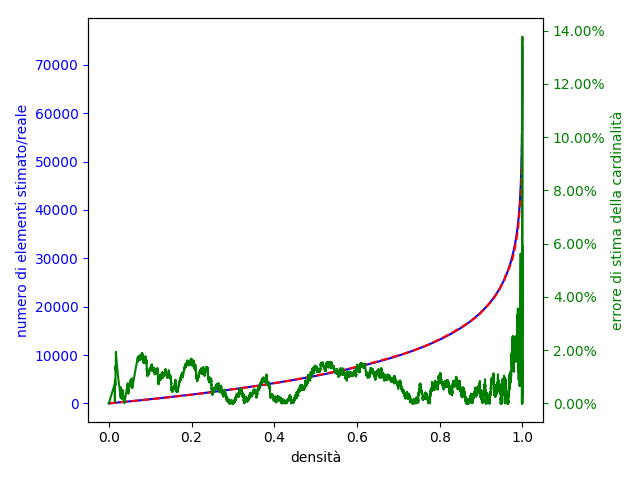
\includegraphics[width=\textwidth]{img/bloom_card_error_1h}
		}
	\end{minipage}
	\qquad
	\begin{minipage}[c]{0.7\textwidth}
		\subfloat[][M=8192, K=2]{
			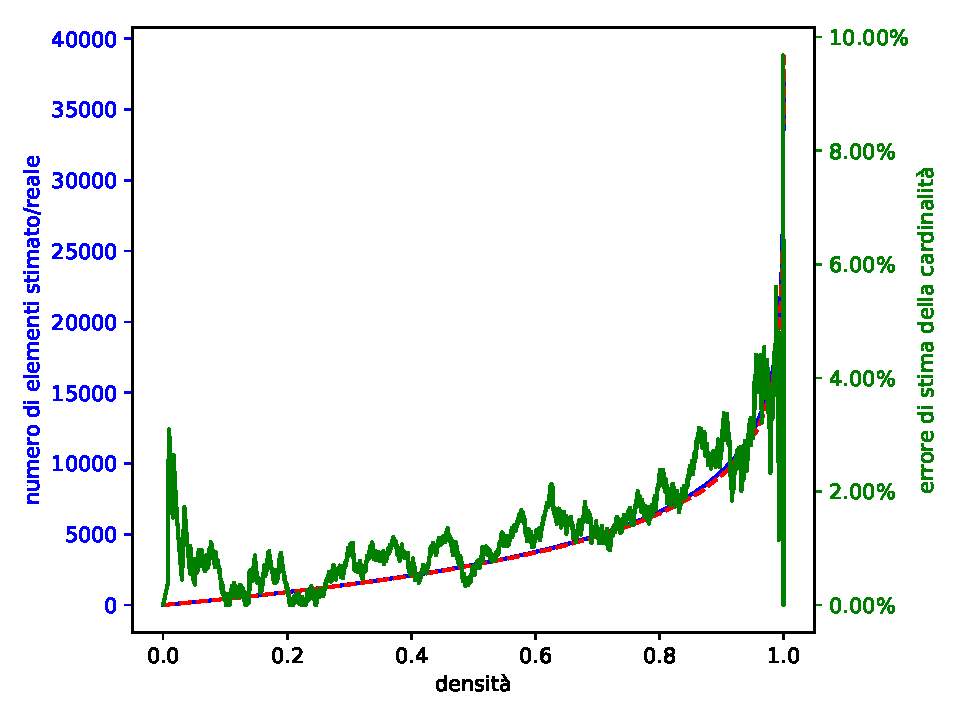
\includegraphics[width=\textwidth]{img/bloom_card_error_2h}
		}
	\end{minipage}
	\qquad
	\begin{minipage}[c]{0.7\textwidth}
		\subfloat[][M=8192, K=3]{
			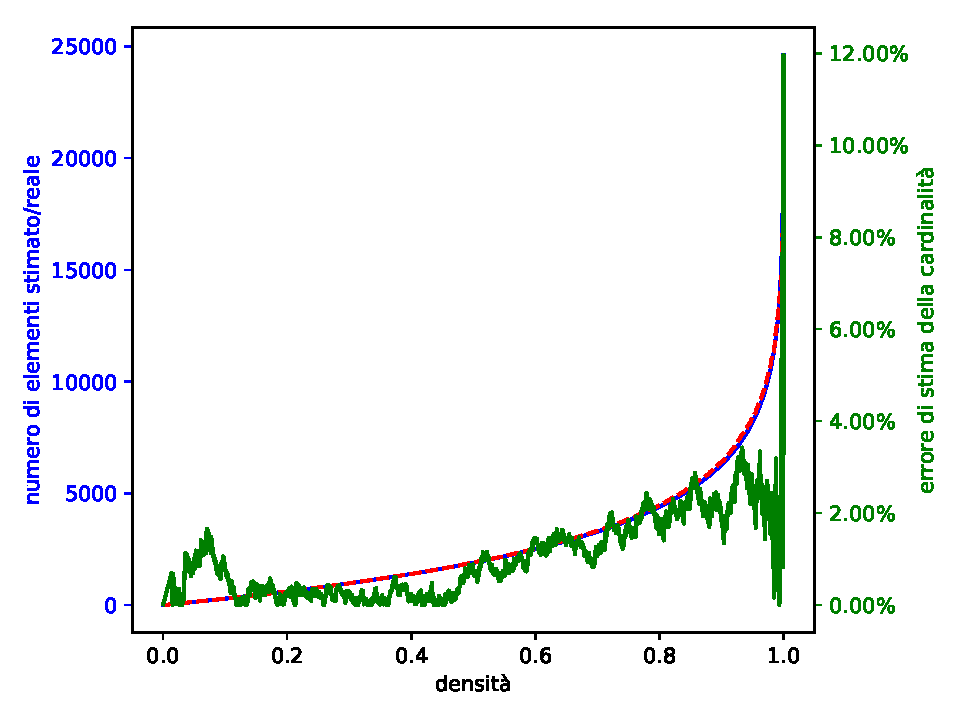
\includegraphics[width=\textwidth]{img/bloom_card_error_3h}
		}
	\end{minipage}

	\caption{Errore sulla cardinalità nei filtri di Bloom commesso dall'\autoref{eq:bloomcard}}
	\label{fig:bloomerror}
\end{figure}

\subsection{Unione ed intersezione}

Dati due filtri creati con gli stessi parametri ed utilizzanti le stesse funzioni di hash, è
possibile calcolare l'unione come mostrato nell'\autoref{alg:bloomunion}, semplicemente applicando
l'operazione di \verb|OR| bit a bit agli array. Questa operazione non causa alcuna perdita di
informazione né pessimizzazione, poiché l'array risultante è il medesimo che si sarebbe ottenuto
aggiungendo in un solo filtro tutti gli elementi presenti nel primo e nel secondo filtro in input.

\begin{algorithm}
\caption{Unione di due filtri di bloom}
\label{alg:bloomunion}
\begin{algorithmic}[1]
\Require $bf_1$ e $bf_2$ devono essere costruiti con gli stessi parametri
\Procedure{BloomUnion}{$bf_1$, $bf_2$}
	\For {$i=0$ \textbf{to} $M-1$}
		\State $out(i) \gets bf_1(i) \lor bf_2(i)$
	\EndFor
	\State \Return $out$
\EndProcedure
\end{algorithmic}
\end{algorithm}


È possibile in modo simile calcolare l'intersezione tra due filtri applicando l'operazione di
\verb|AND| bit a bit agli array, come nell'\autoref{alg:bloomintersection}. In questo caso però
il risultato non è ottimale: l'array risultante potrebbe contenere alcuni bit impostati a 1 che non
risulterebbero tali se si fosse creato direttamente un filtro aggiungendo solo gli elementi facenti
parte dell'intersezione, e di conseguenza la probabilità di falsi positivi risultante dal filtro
intersezione è potenzialmente non ottimale.

\begin{algorithm}
\caption{Intersezione di due filtri di bloom}
\label{alg:bloomintersection}
\begin{algorithmic}[1]
\Require $bf_1$ e $bf_2$ devono essere costruiti con gli stessi parametri
\Procedure{BloomIntersect}{$bf_1$, $bf_2$}
	\For {$i=0$ \textbf{to} $m-1$}
		\State $out(i) \gets bf_1(i) \land bf_2(i)$
	\EndFor
	\State \Return $out$
\EndProcedure
\end{algorithmic}
\end{algorithm}

Supponiamo per esempio di avere due filtri che contengono rispettivamente gli elementi $\{ A, B \}$
e $\{ A, C \}$. Le funzioni di hash sugli elementi sono le seguenti:

\begin{center}
	\begin{tabular}{ l c c c }
		 & A & B & C \\
		\hline
		$h_1(x)$ & 5 & 2 & 7 \\
		$h_2(x)$ & 9 & 6 & 2 \\	
		\hline
	\end{tabular}
\end{center}

I filtri risultanti saranno i seguenti:

\begin{center}
  \begin{tabular}{*{11}{|c}|}
  	\multicolumn{1}{c}{0} & \multicolumn{1}{c}{1} & \multicolumn{1}{c}{2} &
  	\multicolumn{1}{c}{3} & \multicolumn{1}{c}{4} & \multicolumn{1}{c}{5} &
  	\multicolumn{1}{c}{6} & \multicolumn{1}{c}{7} & \multicolumn{1}{c}{8} &
  	\multicolumn{1}{c}{9} & \multicolumn{1}{c}{10} \\
    \hline
    0 & 0 & B & 0 & 0 & A & B & 0 & 0 & A & 0 \\
    \hline
  \end{tabular}
\end{center}

\begin{center}
  \begin{tabular}{*{11}{|c}|}
  	\multicolumn{1}{c}{0} & \multicolumn{1}{c}{1} & \multicolumn{1}{c}{2} &
  	\multicolumn{1}{c}{3} & \multicolumn{1}{c}{4} & \multicolumn{1}{c}{5} &
  	\multicolumn{1}{c}{6} & \multicolumn{1}{c}{7} & \multicolumn{1}{c}{8} &
  	\multicolumn{1}{c}{9} & \multicolumn{1}{c}{10} \\
    \hline
    0 & 0 & C & 0 & 0 & A & 0 & C & 0 & A & 0 \\
    \hline
  \end{tabular}
\end{center}

dove ogni cella impostata a 1 viene identificata con una lettera che si riferisce all'elemento che
l'ha impostata durante l'inserimento. 

L'insieme unione è $\{ A, B \} \cup \{ A , C \} = \{ A, B, C \}$, e il filtro risultante
dall'operazione di \verb|OR| bit a bit, come si può vedere, è ottimale poiché è lo stesso che
avremmo ottenuto per inserimento diretto:

\begin{center}
  \begin{tabular}{*{11}{|c}|}
  	\multicolumn{1}{c}{0} & \multicolumn{1}{c}{1} & \multicolumn{1}{c}{2} &
  	\multicolumn{1}{c}{3} & \multicolumn{1}{c}{4} & \multicolumn{1}{c}{5} &
  	\multicolumn{1}{c}{6} & \multicolumn{1}{c}{7} & \multicolumn{1}{c}{8} &
  	\multicolumn{1}{c}{9} & \multicolumn{1}{c}{10} \\
    \hline
    0 & 0 & B,C & 0 & 0 & A & B & C & 0 & A & 0 \\
    \hline
  \end{tabular}
\end{center}

L'insieme intersezione è $\{ A, B \} \cap \{ A , C \} = \{ A \}$, ma il filtro risultante
dall'operazione di \verb|AND| bit a bit è il seguente:

\begin{center}
  \begin{tabular}{*{11}{|c}|}
  	\multicolumn{1}{c}{0} & \multicolumn{1}{c}{1} & \multicolumn{1}{c}{2} &
  	\multicolumn{1}{c}{3} & \multicolumn{1}{c}{4} & \multicolumn{1}{c}{5} &
  	\multicolumn{1}{c}{6} & \multicolumn{1}{c}{7} & \multicolumn{1}{c}{8} &
  	\multicolumn{1}{c}{9} & \multicolumn{1}{c}{10} \\
    \hline
    0 & 0 & B,C & 0 & 0 & A & 0 & 0 & 0 & A & 0 \\
    \hline
  \end{tabular}
\end{center}
	
Il bit 2 rimane acceso a causa di un conflitto tra le funzioni di hash ($h_1(B) = h_2(C)$), ma
né l'elemento $B$ né l'elemento $C$ sono presenti nell'insieme intersezione. Se il filtro fosse
stato creato da zero, inserendo solamente $A$, il bit 2 risulterebbe impostato a zero.

\section{Ottimizzazione dei parametri}
\label{sec:bloomparms}

Ci sono diversi parametri di interesse quando si analizza un filtro di Bloom, riassunti in questa
tabella.

\medskip
\begin{tabular}{ |l|l| }
  \hline
  \multicolumn{2}{|c|}{Parametri} \\
  \hline
  $M$ & Dimensione in bit dell'array \\
  $K$ & Numero delle funzioni di hash (e delle sezioni) \\
  $m$ & Dimensione in bit di una sezione \\
  $N$ & Numero di elementi presenti nel filtro \\
  $p$ & Densità \\
  $P$ & Probabilità di un falso positivo \\
  \hline
\end{tabular}

\medskip

Vediamo ora come è possibile ottimizzare i parametri, cercando di minimizzare $P$, la probabilità
di un falso positivo, come descritto in \cite{bloom-scalable}.

La probabilità di trovare un bit impostato a 1 in una sezione è $p$, di conseguenza la probabilità 
di un falso positivo, cioè di trovare i bit di tutte le sezioni già impostati, è:

$$ P = p^K $$

Ricordando che $M=km$, otteniamo:

$$ m = M\frac{\ln(p)}{\ln(P)} $$

e sostituendo nella formula della cardinalità, otteniamo:

$$ N \approx -M\frac{\ln(p)\ln(1-p)}{\ln(P)} $$

Supponiamo ora di fissare $M$ (dimensione del filtro) e $P$ (probabilità di un falso positivo), e di
voler cercare qual è la densità $p$ che massimizza il numero di elementi presenti nell'array. È
facile convincersi che il massimo della funzione $\ln(p)\ln(1-p)$ si trova con $p=0.5$, risultato
che ci indica che il punto di utilizzo ottimo di un filtro di Bloom è quando la densità è
esattamente al 50\%, cioè metà dei bit è impostato a 1.

Sostituendo quindi $p=0.5$ come valore ottimo, otteniamo:

$$ N \approx -M\frac{\ln(0.5)^2}{\ln(P)} $$
\begin{equation} \label{eq:bloomn}
N \approx \ceil*{M\frac{0.480453014}{|\ln(P)|}}
\end{equation}

che ci permette di calcolare il numero di elementi memorizzabili in un filtro prima di raggiungere
la densità di 0.5 e dunque la probabilità $P$ di falsi positivi richiesta. Oppure, ricavando
le altre variabili:

\begin{equation} \label{eq:bloomm}
M = \ceil*{n\frac{|\ln(P)|}{0.480453014}} 
\end{equation}
\begin{equation} \label{eq:bloomp}
P = e^{-\ln(0.5)^2\frac{M}{N}} = 0.5^{\ln(2)\frac{M}{N}} \approx 0.6185^{\frac{M}{N}}
\end{equation}

possiamo calcolare la dimensione ottimale di un filtro dato il numero di elementi che si vuole
memorizzare e la probabilità di falsi positivi attesa, oppure ancora i falsi positivi attesi
data la dimensione di un filtro e il numero di elementi inseriti. 

Inoltre, da $P = p^k$, sostituendo nuovamente $p=0.5$, possiamo ricavare:

\begin{equation} \label{eq:bloomk}
 K = \ceil*{\log_2{\frac{1}{P}}} = \ceil*{-\log_2{P}}
\end{equation}

con cui calcolare il numero ottimale di funzioni di hash per un data probabilità attesa di falso
positivo.

Vediamo ora due esempi di derivazione di parametri ottimali. 

\begin{itemize}
	\medskip

	\item Supponiamo di voler memorizzare $N=\num{25000}$ elementi in un filtro con una probabilità di
	falso positivo $P=\SI{0.5}{\percent}$; possiamo ricavare i parametri necessari in questo modo:

	$$ M = \ceil*{n\frac{|\ln(P)|}{0.480453014}} = \ceil*{25000\frac{|\ln(0.005)|}{0.480453014}} = \num{275694} $$
	$$ K = \ceil*{-\log_2{P}} = \ceil*{-\log_2{0.005}} = 8 $$

	Quindi è necessario utilizzare un filtro di circa \SI{33}{\kibi\byte} con \num{8} funzioni di hash.

	\item Supponiamo di avere \SI{1}{\mebi\byte} di RAM a disposizione per creare un filtro di Bloom che deve
	memorizzare 2 milioni di elementi. Qual è il valore minimo di falso positivo che possiamo
	ottenere, e con quante funzioni di hash lo otterremo? È presto detto:

	$$ M = \num{1024 x 1024 x 8} = \num{8388608} $$
	$$ N = \num{2000000} $$
	$$ P = 0.6185 ^ \frac{M}{N} \approx 0.1463 \approx \SI{15}{\percent} $$
	$$ K = \ceil*{-\log_2{P}} = 3 $$

	Quindi possiamo arrivare ad avere circa il \SI{15}{\percent} di falsi positivi utilizzando
	\num{3} funzioni di hash.
\end{itemize}

\begin{figure}
	\centering
	\begin{minipage}[c]{\textwidth}
		\subfloat[][Numero di elementi in base alla probabilità attesa]{
			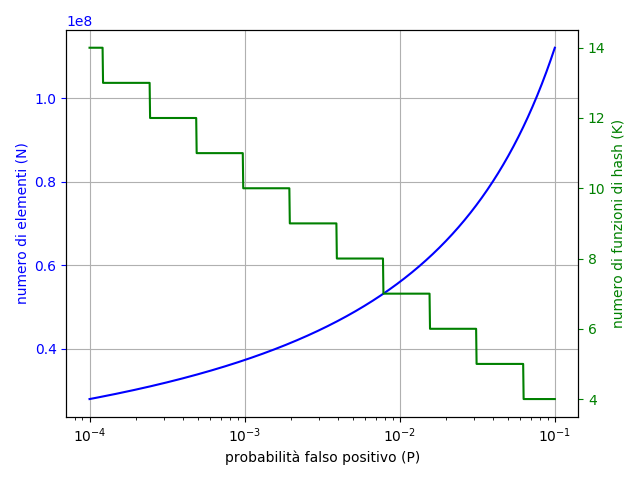
\includegraphics[width=\textwidth]{img/bloom_parms_1}
		}
	\end{minipage}
	\qquad
	\begin{minipage}[c]{\textwidth}
		\subfloat[][Probabilità attesa in base al numero di elementi]{
			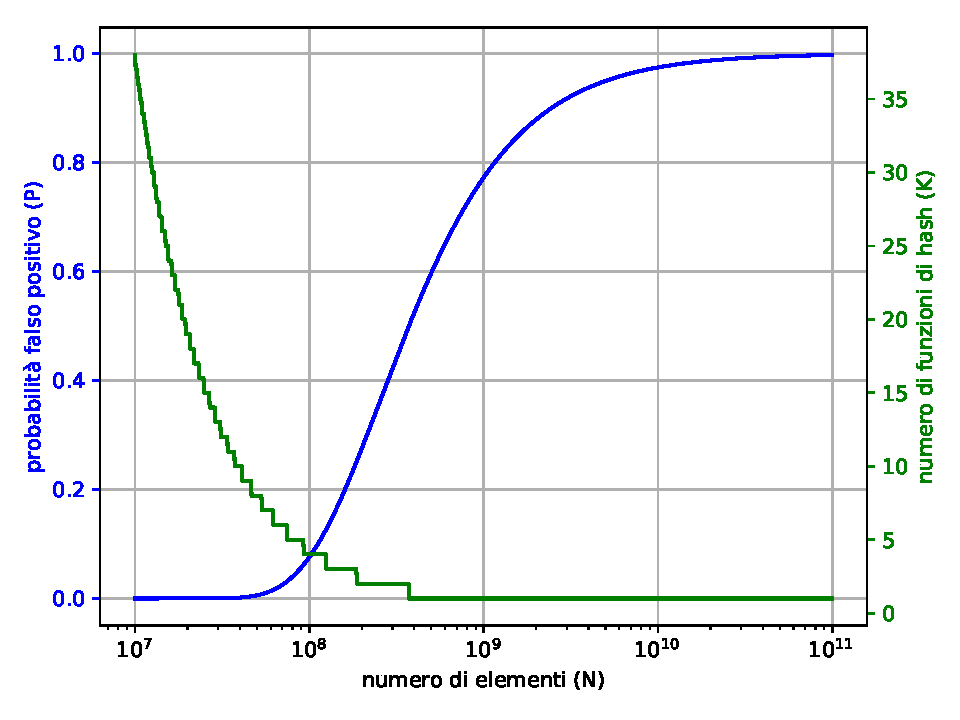
\includegraphics[width=\textwidth]{img/bloom_parms_2}
		}
	\end{minipage}

	\caption{Andamento dei parametri ottimale in un filtro di \SI{64}{\mebi\byte}}
\end{figure}

\section{Filtri scalabili}
\label{sec:bloomscalable}

Uno dei problemi principali dei filtri così come originariamente progettati è che la struttura
dati è definita staticamente, e dunque non è possibile espanderla dinamicamente in base al
numero di elementi che via via si rende necessario memorizzare. Questo limite rende complesso
l'utilizzo in diversi scenari applicativi, poiché, volendo mantenere la probabilità di un falso
positivo contenuta entro una soglia, è necessario spesso sovradimensionare il filtro a causa della 
impossibilità di prevedere il numero di elementi che sarà necessario memorizzare.

Per risolvere questo problema, \cite{bloom-scalable} propone di creare un \emph{filtro di Bloom
scalabile} (SBF) formato da uno o più filtri in catena; quando i filtri raggiungono la densità
scelta come obiettivo (di solito $p=0.5$), un nuovo filtro viene aggiunto in coda alla catena,
facendo spazio così per l'inserimento nuovi elementi. Il test di appartenenza dovrà quindi ricercare
l'elemento all'interno di tutti i filtri della catena. Ogni filtro che viene creato avrà una nuova
probabilità $P_j$ per i falsi positivi, seguendo una progressione geometrica ($P_i = rP_{i-1} =
r^iP_0$), in modo che la probabilità composta $P$ dell'intera catena converga verso il valore
richiesto. Il fattore $r \in \interval[open]{0}{1}$ è detto \emph{fattore di intensificazione}
(``tighten ratio'').

La probabilità composta $P$, ottenuta ricercando l'elemento negli $l$ filtri della catena, può
essere quindi calcolata così:

$$ P = 1 - \prod_{i=0}^{l-1}(1-r^iP_0) $$

e volendo calcolare un limite superiore, possiamo ottenere:

$$ P \leq \sum_{i=0}^{l-1} r^iP_0 \leq \lim_{l \rightarrow \infty} \sum_{i=0}^{l-1} r^iP_0 =
\frac{1}{1-r}P_0 $$

Ricavando $P_0$, possiamo calcolare il valore di probabilità di falsi positivi che deve avere
il primo filtro della catena, in base al fattore di intensificazione $r$ e la probabilità finale
attesa $P$:

\begin{equation} \label{eq:p0fromp}
P_0 = (1-r)P
\end{equation}

Possiamo anche calcolare il numero ottimale di funzioni di hash che deve usare ogni filtro nella
catena:

$$ k_0 = -\log_2{P_0} $$
$$ k_i = -\log_2{P_i} = -\log_2{(r^iP_0)} = k_0 + i \log_2{\frac{1}{r}} $$

Per quanto concerne invece la dimensione $M_i$ dei filtri, è consigliabile utilizzare anche qui
una progressione geometrica (il cui fattore è chiamato $s$), che si adatta velocemente ad una
crescita importante di elementi nel filtro senza aumentare troppo la lunghezza della catena (che
impatterebbe sulla velocità del test di appartenenza). 

Per quanto concerne i valori ottimali dei parametri $r$ e $s$, rimandiamo a \cite{bloom-scalable} per
l'analisi sperimentale che mostra che i valori ottimali di $r$ sono $r \in \interval{0.8}{0.9}$,
mentre il parametro $s$ può essere usato normalmente con valore \num{2}, aumentando magari a \num{4}
se si prevede un numero molto elevato di elementi.

